\pdfoptionpdfminorversion = 7
\documentclass[UTF8]{book}
\usepackage[T1]{fontenc}

\usepackage{pdfpages}
\usepackage{ctex}
\usepackage{tikz}
\usepackage{graphicx}
\usepackage{fancyhdr}
% \usepackage{ifpdf}              % if pdflatex then ... else ...
% \ifpdf
%  \pdfadjustspacing=1           % make pdflatex behave like latex
%  \usepackage{aeguill}          % PS converted CM fonts for better acro preview
%  \usepackage[pdftex]{graphicx} % graphics packages
%  \usepackage[pdftex]{color}    % color packages
%  \usepackage[pdftex]{thumbpdf} % create thumbnails (run thumbpdf as well)
%  \pdfoptionpdfminorversion = 7

\usepackage[backref]{hyperref}




\begin{document}
	\pagestyle{fancy}
    
	\chapter{配送员盘点}
	
	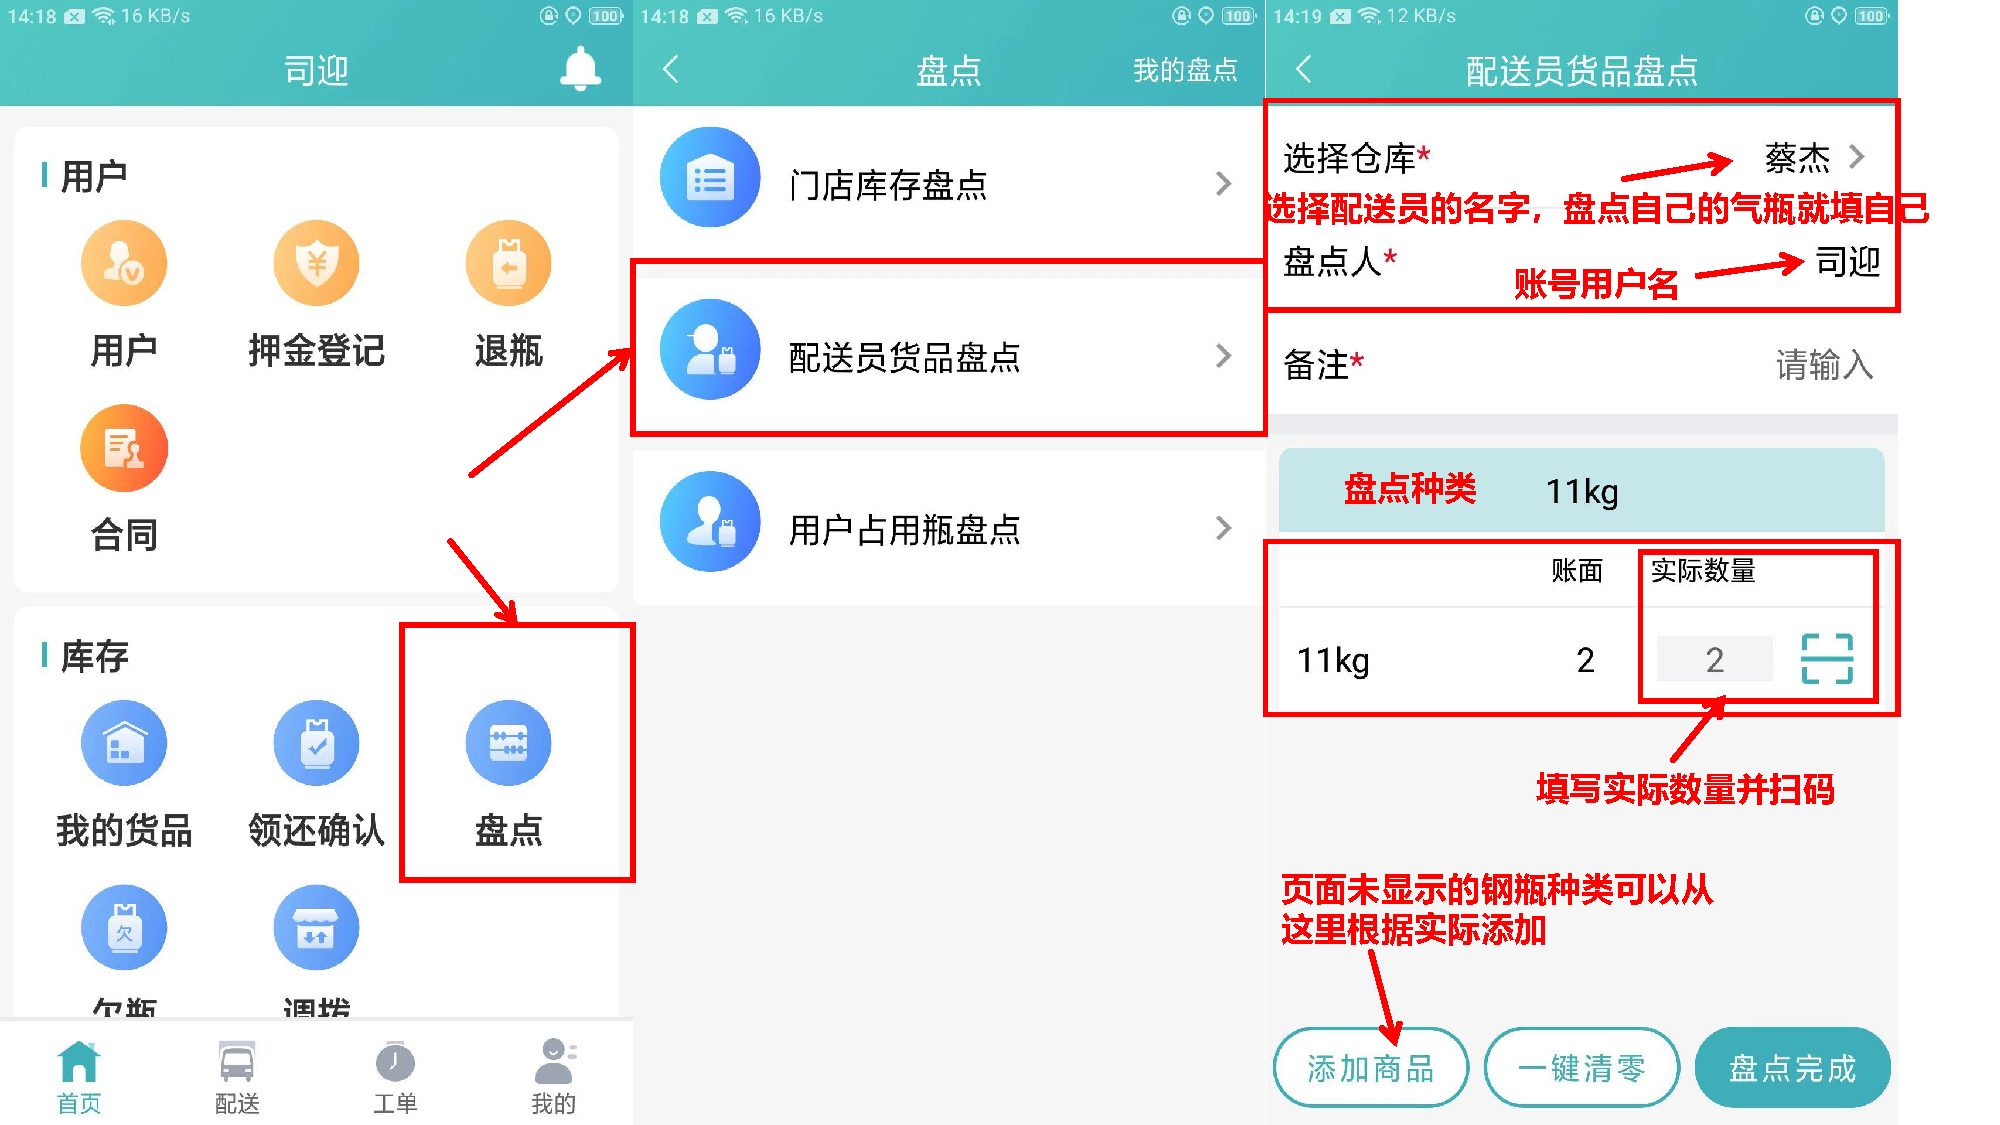
\includepdf[pages={1-},nup=1x2]{./haoyunqi_tutorial_pdfs/delivery_stock}

	\chapter{接单与收押金}
	
	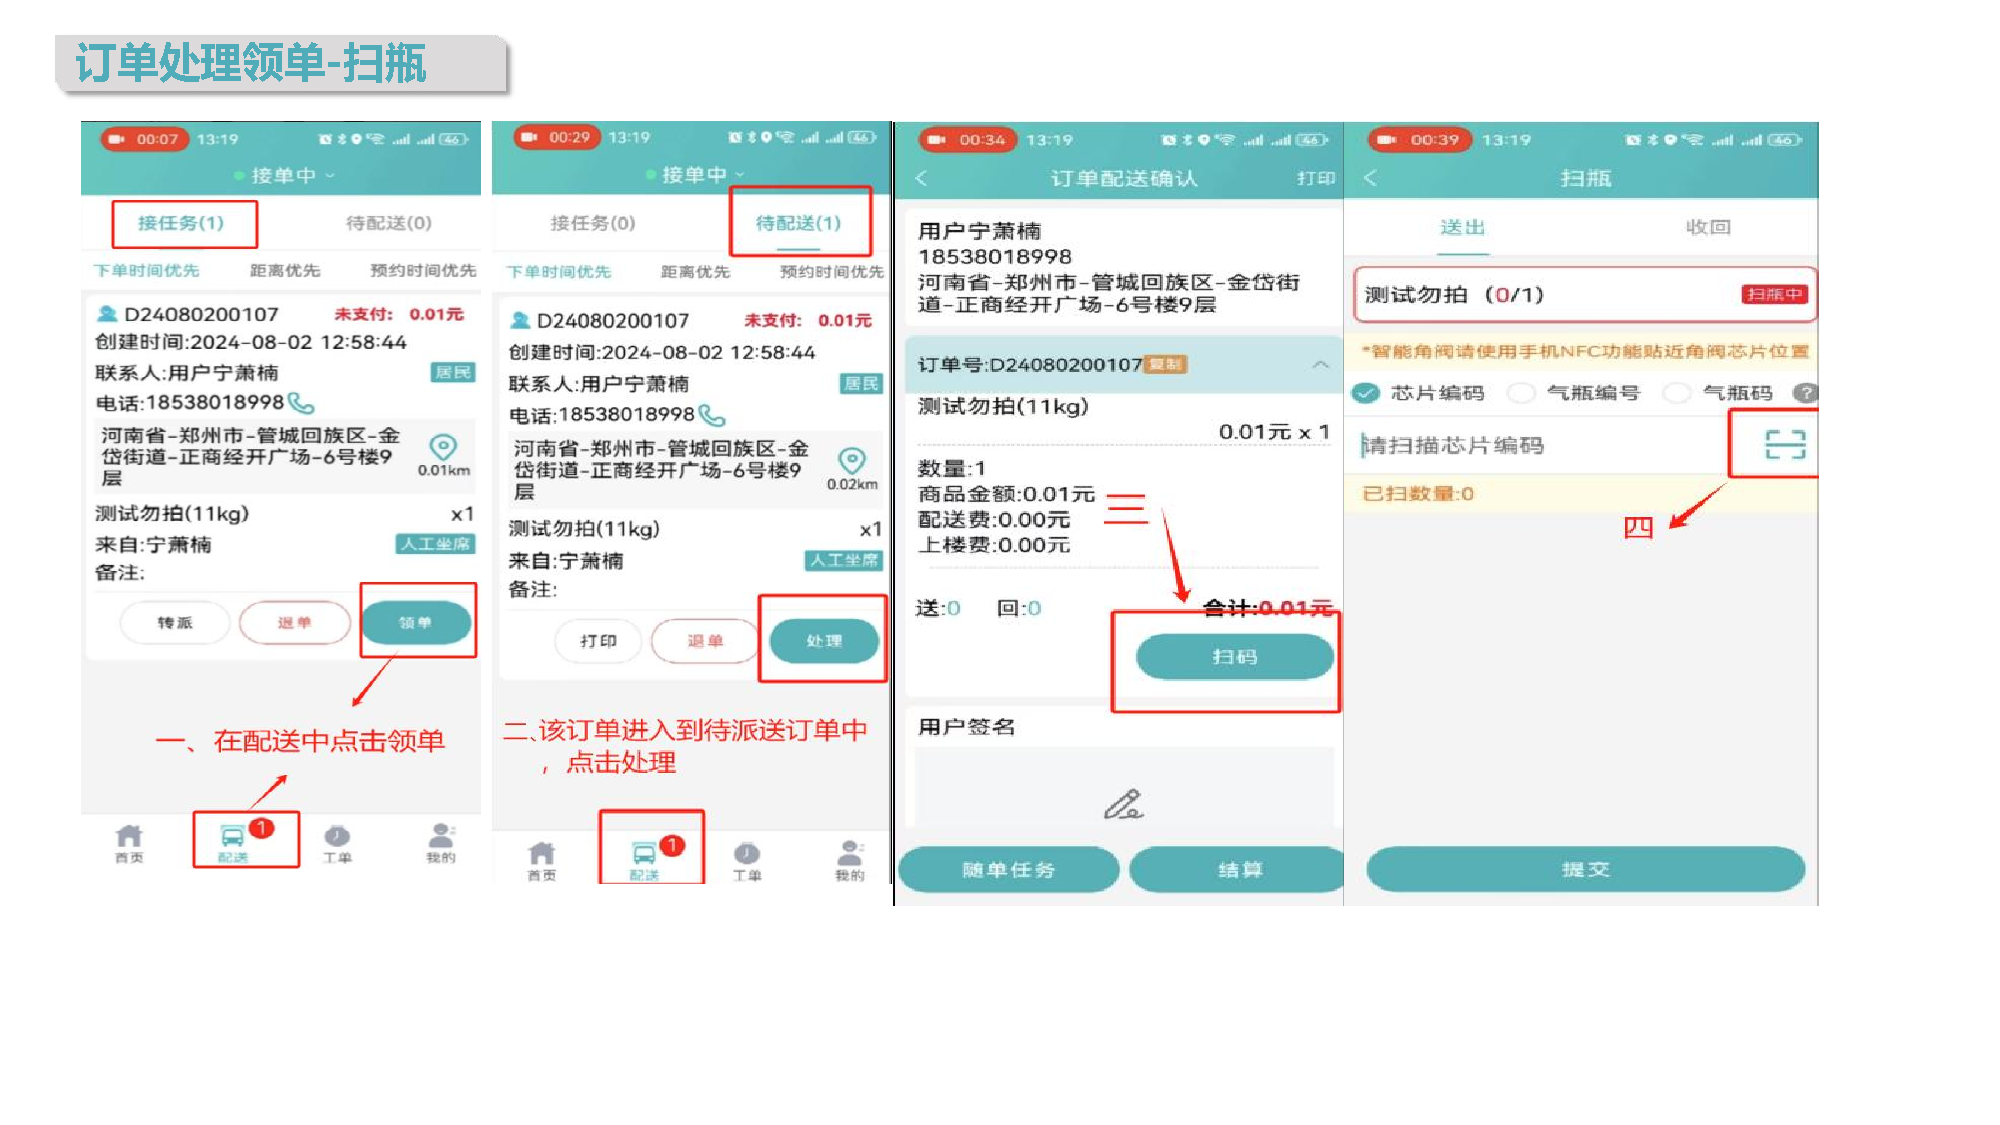
\includepdf[pages={1-4},nup=1x2,width=1.8\linewidth,height=0.7\textheight]{./haoyunqi_tutorial_pdfs/taking_orders_deposit}
	
	\chapter{app修改用户信息}
	
	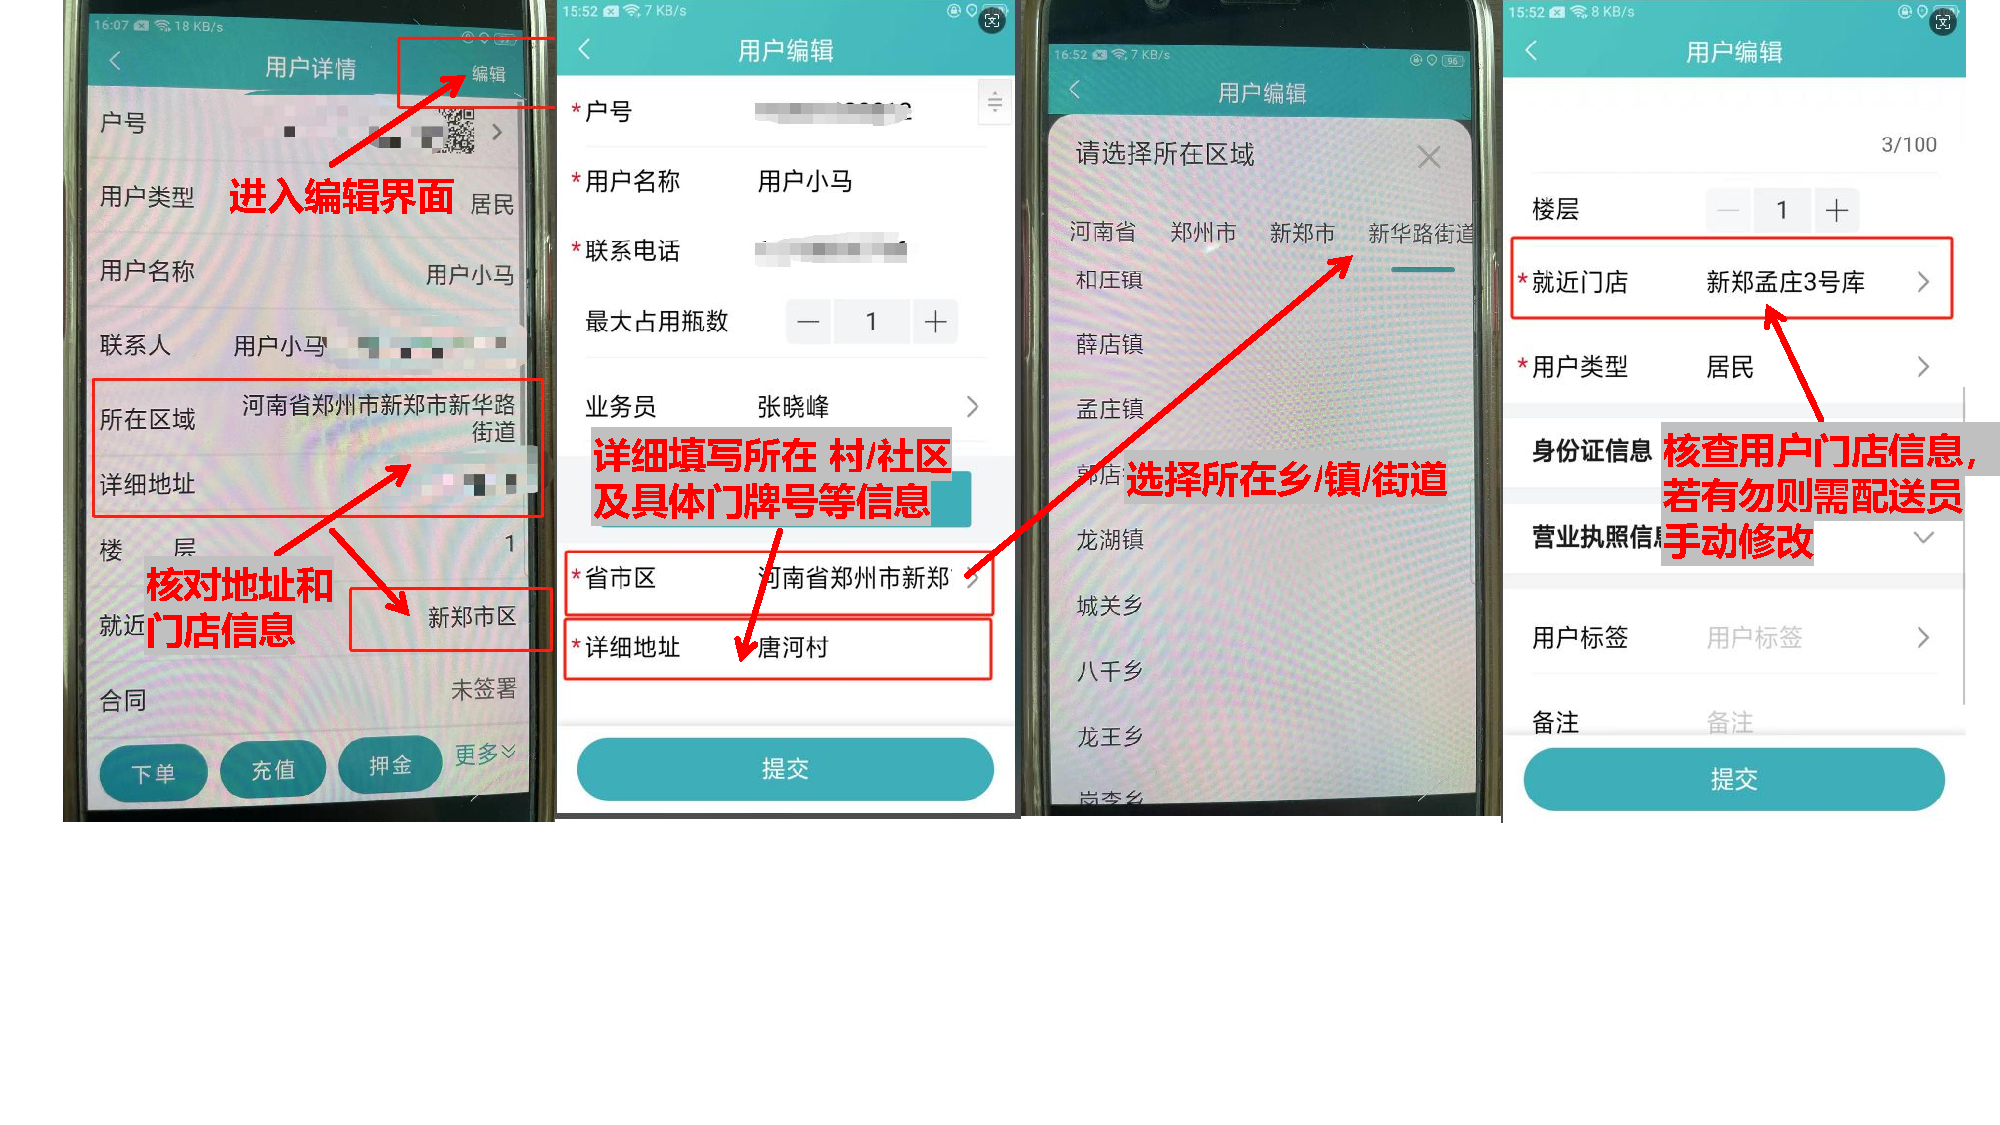
\includepdf[pages={1-}]{./haoyunqi_tutorial_pdfs/app_modify_user_dep}
	
	\chapter{网页端补押金单}
	
	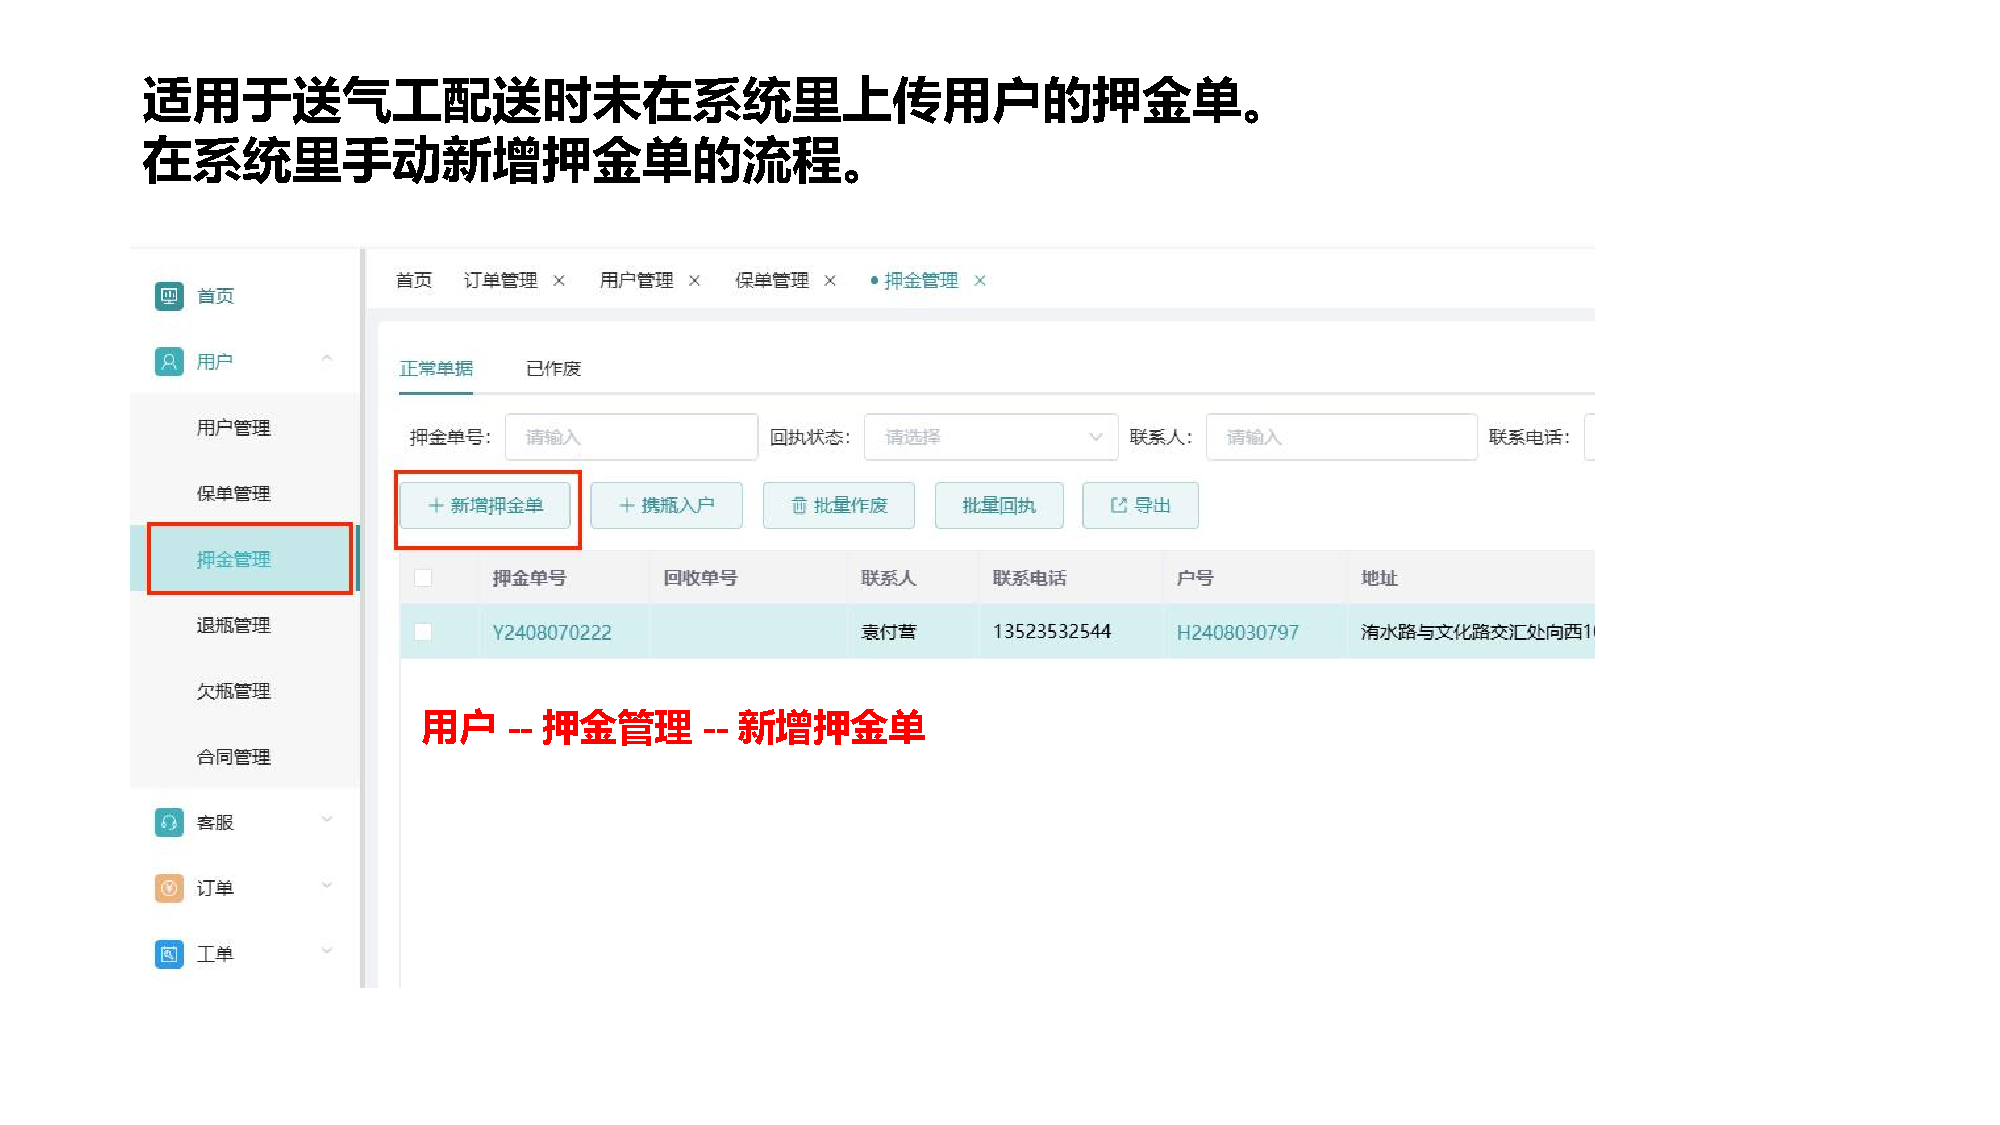
\includepdf[pages={1-},nup=1x2]{./haoyunqi_tutorial_pdfs/make_up_deposit}
	
	\chapter{营业员调拨车单与司机装卸车扫码}
	
	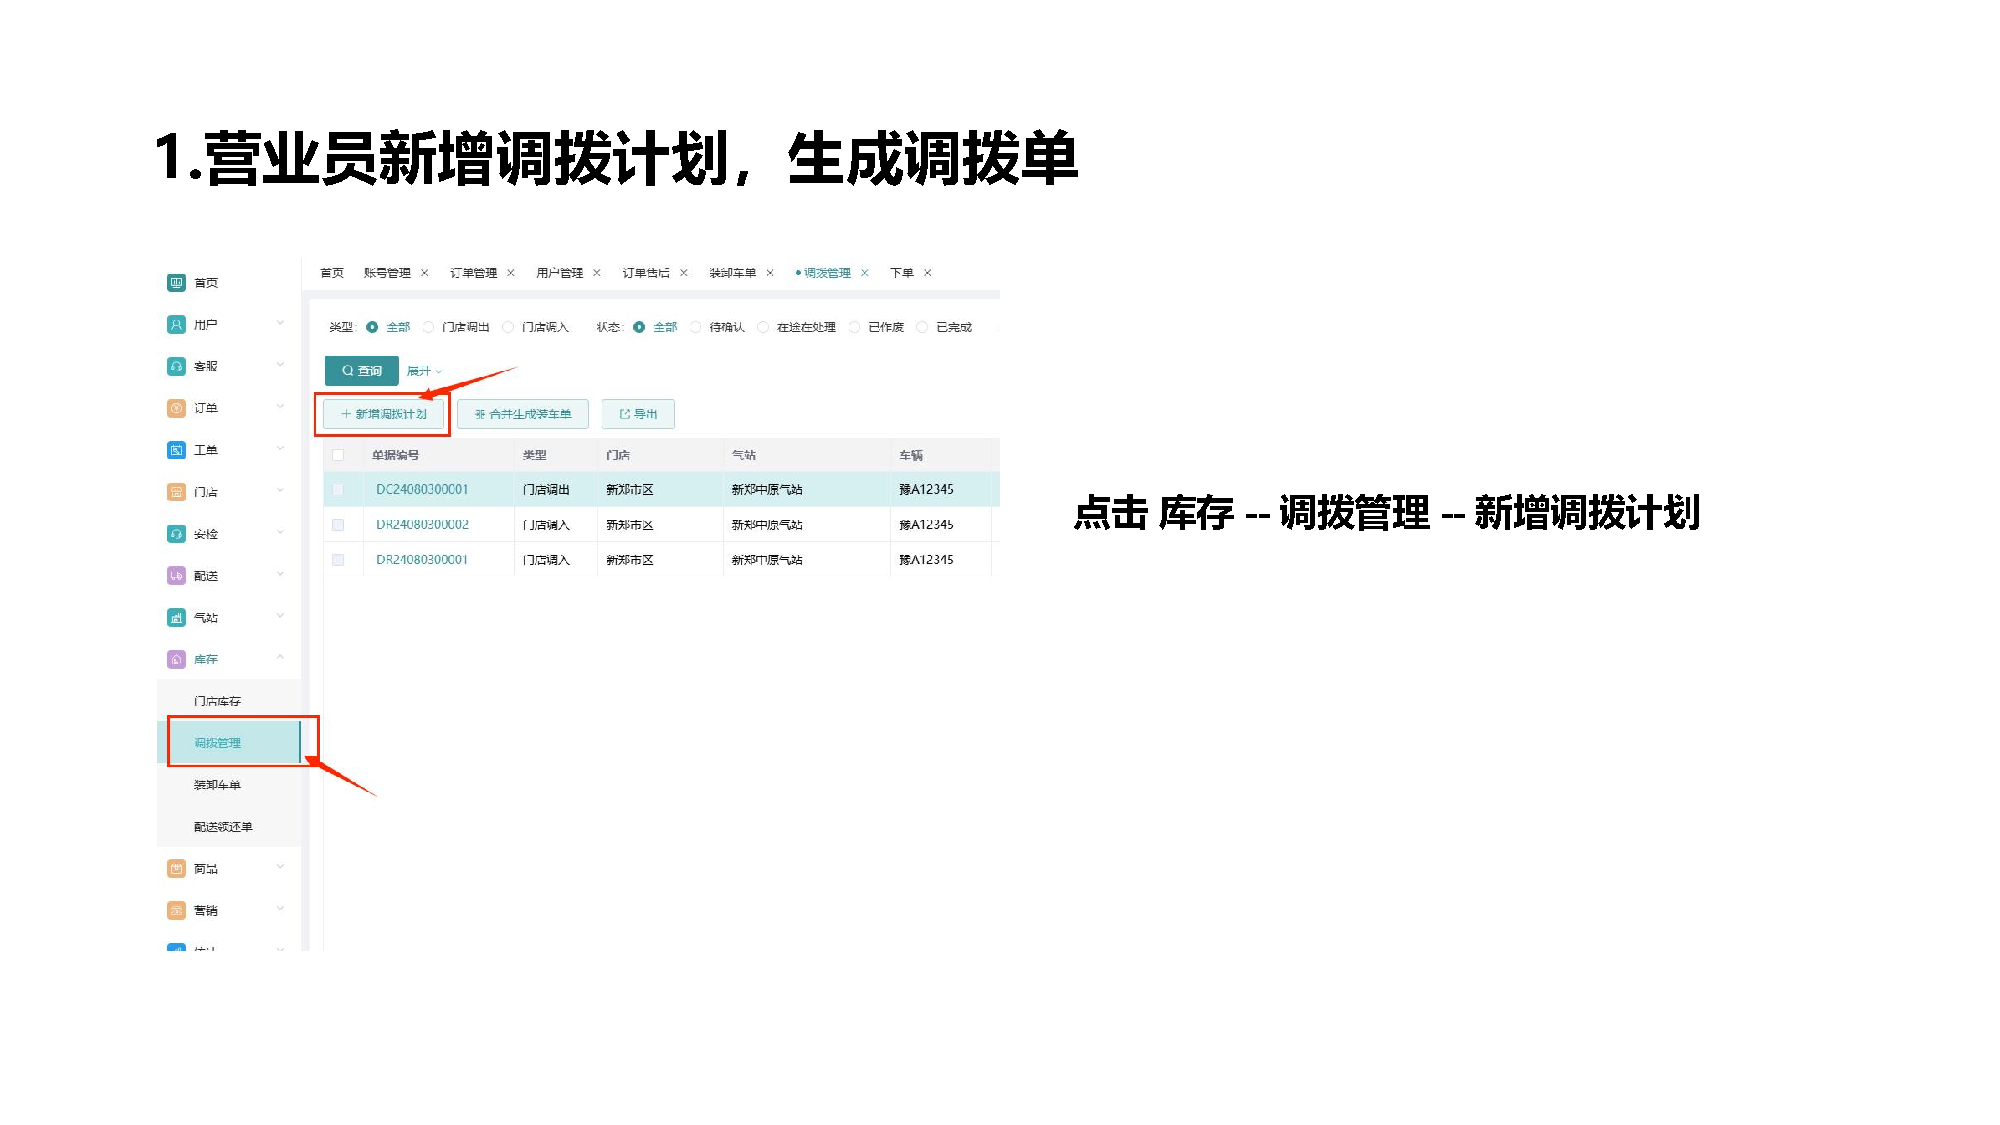
\includepdf[pages={1-},nup=1x2,width=1.8\linewidth,height=0.7\textheight]{./haoyunqi_tutorial_pdfs/agency_stock}
	
	

\end{document}